\documentclass[a4paper, 12pt, oneside, dvipsnames, table]{article}
\usepackage{../../Utilita/Stiletemplate}
\usepackage{hyperref}
\usepackage{fancyhdr}
\usepackage[italian]{babel}
\usepackage[utf8]{inputenc}
\usepackage{float}
\usepackage{siunitx}
\usepackage{comment}
\restylefloat{table}

\newcommand{\Data}{2021\_01\_30}

\newcommand{\Titolo}{Verbale riunione \Data}

\newcommand{\Redattori}{\TL}

\newcommand{\Verificatori}{\PC}

\newcommand{\Approvatore}{\VD}

\newcommand{\Distribuzione}{\VT{} \newline \CR{} \newline Gruppo \Gruppo}

\newcommand{\Uso}{Interno}

\newcommand{\DescrizioneDoc}{Questo documento si occupa di riportare quanto discusso nella riunione del \Data.}

\newcommand{\pathimg}{../../../Immagini/N.O.S.jpg}

\newcommand{\Versionedoc}{1.0}
% info generali 
\newcommand{\NomeProgetto}{\textit{Emporio$\lambda$ambda}}

% fornitore
\newcommand{\Gruppo}{\textit{N.O.S}}
\newcommand{\Mail}{nos.unipd@gmail.com}

% committenti
\newcommand{\Committente}{\VT \newline \CR}
\newcommand{\VT}{Prof. Vardanega Tullio}
\newcommand{\CR}{Prof. Cardin Riccardo}

% proponenti
\newcommand{\Proponente}{\textit{RedBabel}}

% Componenti
\newcommand{\BL}{Brescanzin Lorenzo}
\newcommand{\FF}{Fantinato Filippo}
\newcommand{\MM}{Martini Matteo}
\newcommand{\PC}{Panighel Cristiano}
\newcommand{\TG}{Terrani Giulia}
\newcommand{\TL}{Tredese Leonardo}
\newcommand{\VD}{Varotto Davide}

% ruoli

\newcommand{\Responsabile}{\textit {Responsabile di Progetto}}
\newcommand{\Amministratore}{\textit{Amministratore di Progetto}}

% documenti

\newcommand{\SdF}{Studio di Fattibilità}
\newcommand{\SdFv}[1]{\textit{Studio di Fattibilità {#1}}}
\newcommand{\PdQ}{Piano di Qualifica}
\newcommand{\PdQv}[1]{\textit{Piano di Qualifica {#1}}}
\newcommand{\PdP}{Piano di Progetto}
\newcommand{\PdPv}[1]{\textit{Piano di Progetto {#1}}}
\newcommand{\NdP}{Norme di Progetto}
\newcommand{\NdPv}[1]{\textit{Norme di Progetto {#1}}}
\newcommand{\AdR}{Analisi dei Requisiti}
\newcommand{\AdRv}[1]{\textit{Analisi dei Requisiti {#1}}}
\newcommand{\Glossario}{Glossario}
\newcommand{\Glossariov}[1]{\textit{Glossario {#1}}}

% comandi generali
\newcommand{\glo}[1]{#1\ap{G}}

\newcommand{\myparagraph}[1]{\paragraph{#1}\mbox{}\\}

\setcounter{tocdepth}{5}  \setcounter{secnumdepth}{5}

	
\begin{document}

\copertina{}
\newpage

\fancydoc{}
\registroModifiche{
	
	2.0 & 2021\_03\_06 & \VD{} & Responsabile & - & Approvazione del documento. \\
	
	1.20 & 2021\_03\_05 & \MM{} & Analista & \TL{} & Inseriti UML corretti. \\
	
	1.19 & 2021\_03\_04 & \PC{} & Analista & \TL{} & Aggiornata sezione \S\ref{Tracciamento}. \\
	
	1.18 & 2021\_03\_02 & \PC{} & Analista & \BL{} & Aggiornata sezione \S\ref{ReqFunz}, requisiti del venditore. \\
	
	1.17 & 2021\_03\_01 & \MM{} & Analista & \PC{} & Aggiornata sezione \S\ref{ReqFunz}, requisiti dell'acquirente. \\
	
	1.16 & 2021\_02\_26 & \BL{} & Analista & \PC{} & Correzione dei precedenti e aggiunta di nuovi UC, estensioni di UC già presenti. \\

	1.15 & 2021\_02\_25 & \TG{} & Analista & \PC{} & Correzione UC "Lista riepilogo ordini" ora UC\ref{visualizzazione-ordini-in-gestione} e aggiunta UC da UC\ref{modifica-stato-ordine} a UC\ref{filtro-ordini-venditore}. \\
	
	1.14 & 2021\_02\_24 & \TG{} & Analista & \FF{} & Redatti nuovi UC\ref{ricerca-codice-ordine-acquirente} e UC\ref{filtro-temporale-ordini-acquirente}.\\
	
	1.13 & 2021\_02\_21 & \TG{} & Analista & \FF{} & Redatti nuovi UC\ref{inserimento-indirizzo-consegna}, UC\ref{modifica-indirizzo-consegna} e UC\ref{eliminazione-indirizzo-consegna}. \\
	
	1.12 & 2021\_02\_19 & \MM{} & Analista & \TG{} & Eliminato UC23-"Inserimento campo dati" e UC15-"Modifica informazioni profilo" ora suddiviso in UC\ref{modifica-informazioni-acquirente} e UC\ref{modifica-informazioni-venditore}. \\

	1.11 & 2021\_02\_18 & \PC{} & Analista & \BL{} & Correzione UC\ref{checkout}. \\

	1.10 & 2021\_02\_15 & \BL{} & Analista & \PC{} & Correzioni \S\ref{ReqVincolo} e \S\ref{ReqQual}, da UC\ref{aggiunta-carrello-plp} a UC\ref{modifica-quantita-nel-carrello}.\\
	
	1.9 & 2021\_02\_14 & \BL{} & Analista & \TG & Sistemazione UC\ref{logout} e UC\ref{ricerca-prodotti-acquirente}. \\
	
	1.8 & 2021\_02\_13 & \TG{} & Analista & \MM{} & Aggiunto i casi d'uso UC\ref{aggiunta-categoria}, UC\ref{modifica-categoria}, UC\ref{eliminazione-categoria}. \\

	1.7 & 2021\_02\_10 & \PC{} & Analista & \MM{} & Corretto i caso d'uso UC\ref{aggiunta-prodotto-evidenza} e UC\ref{rimozione-prodotto-evidenza}. \\

	1.6 & 2021\_02\_09 & \TG{} & Analista & \TL{} & Corretto le sezioni UC\ref{aggiunta-prodotto} e UC\ref{modifica-prodotto}. \\
	
	1.5 & 2021\_02\_08 & \MM{} & Analista & \FF{} & Trasformato sottocasi d'uso indipendenti relativi al venditore in casi d'uso. \\
	
	1.4 & 2021\_02\_04 & \MM{} & Analista & \PC{} & Trasformato sottocasi d'uso indipendenti relativi all'acquirente in casi d'uso. \\

	1.3 & 2021\_02\_03 & \TG{} & Analista & \TG{} & Rimossi i dettagli implementativi dai casi d'uso. Eliminato UC3-"Accesso al menù". \\

	1.2 & 2021\_02\_02 & \PC{} & Analista & \TL{} & Separati i casi di accesso alla piattaforma sezione \S\ref{AccessoPiattaforma}. \\

	1.1 & 2021\_02\_02 & \BL{} & Analista & \FF{} & Rimosso l'attore amministratore sezione \S\ref{Attori}. \\ 

	1.0.0 & 2021\_01\_10 & \PC{} & Responsabile & - & Approvazione del documento. \\
	
	0.1.7 & 2021\_01\_09 & \FF{} & Analista & \TL{} & Stesura riepilogo tracciamento \S\ref{Riepilogo} \\
	
	0.1.6 & 2021\_01\_09 & \TL{} & Analista & \BL{} & Stesura tracciamento requisito-fonte \S\ref{ReqFonte} \\
	
	0.1.5 & 2021\_01\_09 & \BL{} & Analista & \FF{} & Stesura tracciamento fonte-requisito \S\ref{FonteReq} \\
	
	0.1.4 & 2021\_01\_08 & \MM{} & Analista & \BL{} & Aggiunta diagrammi dei casi d'uso \S\ref{CasiUso} \\
	
	0.1.3 & 2021\_01\_08 & \TL{} & Analista & \TG{} & Stesura requisiti vincolo \S\ref{ReqVincolo} e prestazionali \S\ref{ReqPrest} \\
	
	0.1.2 & 2021\_01\_08 & \FF{} & Analista & \TG{} & Stesura requisiti di qualità \S\ref{ReqQual} \\
	
	0.1.1 & 2021\_01\_07 & \BL{} & Analista & \TG{} & Stesura requisiti funzionali \S\ref{ReqFunz} \\
	
	0.1.0 & 2021\_01\_06 & - & - & \TG{} & Verifica complessiva del documento. \\
	
	0.0.10  & 2020\_12\_27 & \FF{} & Analista & \TG{} & Stesura caso d'uso UC\ref{estensione:limite-foto-raggiunto}, UC\ref{estensione:prezzo-minore-o-uguale-zero}, UC\ref{estensione:email-non-esistente}, UC\ref{estensione:registrazione-con-email-non-esistente}, UC\ref{estensione:quantita-da-aggiungere-al-carrello-non-valida}, UC\ref{estensione:sconto-minore-zero}, UC\ref{estensione:pagamento-fallito}, UC\ref{estensione:sconto-maggiore-cento} \\
	
	0.0.9 & 2021\_01\_05 & \BL{} & Analista & \TG{} & Stesura casi d'uso: UC\ref{estensione:cambio-con-email-esistente}, UC\ref{estensione:campo-obbligatorio-non-inserito}, UC\ref{estensione:credenziali-non-presenti}, UC\ref{estensione:email-non-valida}, UC\ref{estensione:file-no-tipo-immagine} \\
	
	0.0.8 & 2021\_01\_04 & \TL{} & Analista & \TG{} & Aggiornamento sezioni UC\ref{eliminazione-prodotto}, UC\ref{aggiunta-prodotto-evidenza}, UC\ref{rimozione-prodotto-evidenza}, UC\ref{rifornimento-prodotto} \\
	
	0.0.7 & 2021\_01\_04 & \TL{} & Analista & \TG{} & Aggiornamento sezioni UC\ref{modifica-informazioni-venditore}, UC\ref{eliminazione-account-acquirente}, UC\ref{aggiunta-prodotto}, UC\ref{modifica-prodotto} e \S\ref{Attori} \\
	
	0.0.6 & 2021\_01\_03 & \BL{} & Analista & \TG{} & Stesura casi d'uso: UC\ref{modifica-quantita-da-aggiungere-al-carrello}, UC\ref{eliminazione-prodotto-dal-carrello}, UC\ref{checkout}, UC\ref{visualizzazione-ordini-effettuati}, UC\ref{modifica-informazioni-acquirente} \\
	
	0.0.5  & 2021\_01\_02 & \BL{} & Analista & \TG{} & Stesura casi d'uso: UC\ref{ordinamento-prezzo-decrescente}, UC\ref{aggiunta-carrello-pdp}, UC\ref{aggiunta-carrello-plp} \\
	
	0.0.4  & 2021\_01\_02 & \FF{} & Analista & \TG{} & Stesura casi d'uso: UC\ref{logout}, UC\ref{ricerca-prodotti-acquirente}, UC\ref{filtro-prodotti-acquirente}, UC\ref{ordinamento-prezzo-crescente} \\
	
	0.0.3  & 2021\_01\_01 & \FF{} & Analista & \TG{} & Stesura casi d'uso: UC\ref{registrazione}, UC\ref{autenticazione-acquirente}, UC\ref{autenticazione-venditore}, UC\ref{password-dimenticata} \\ 
	
	0.0.2  & 2020\_12\_27 & \TG{} & Analista & \TL{} & Stesura \S\ref{Desc} \\  
	
	0.0.1  & 2020\_12\_22 & \TG{} & Analista & \BL{} & Stesura scheletro del documento, \S\ref{Intro}, \S\ref{Desc} \\
}

\setcounter{table}{0}

\clearpage
\tableofcontents
\clearpage

\listoftables
\newpage

\listoffigures
\newpage

\section{Introduzione}
\subsection{Scopo del Documento}
Questo documento contiene la stesura dello studio di fattibilità riguardante i sette capitolati proposti, elencando quelli che il nostro gruppo ha considerato come i loro aspetti più interessanti e le loro criticità. Infine, per ogni capitolato vengono esposte le motivazioni e le ragioni per cui il gruppo ha scelto come progetto il capitolato C2 \NomeProgetto{} a discapito degli altri sei proposti.

\subsection{Glossario}
Al fine di evitare ambiguità fra i termini, e per avere le terminologie chiare fra tutti gli stakeholder, il gruppo \Gruppo{} ha redatto un documento denominato \Glossariov{1.0.0}.
In tale documento sono presenti tutti i termini tecnici, ambigui, specifici del progetto e scelti dai membri del gruppo con le loro relative definizioni.
Un termine presente nel \Glossariov{1.0.0} e utilizzato in questo documento viene indicato con un apice \ap{G} alla fine della parola.

\subsection{Riferimenti}

\subsubsection{Normativi}
\begin{itemize}
\item \NdPv{1.0.0}.
\end{itemize}

\subsubsection{Informativi}

\begin{itemize}
\item \textbf {Capitolato d'appalto C1 - BlockCOVID:}\\
\url{https://www.math.unipd.it/~tullio/IS-1/2020/Progetto/C1.pdf}
\item \textbf {Capitolato d'appalto C2 - \NomeProgetto:}\\
\url{https://www.math.unipd.it/~tullio/IS-1/2020/Progetto/C2.pdf}
\item \textbf {Capitolato d'appalto C3 - Gathering Detection Platform:}\\
\url{https://www.math.unipd.it/~tullio/IS-1/2020/Progetto/C3.pdf}
\item \textbf {Capitolato d'appalto C4 - HD Viz:}\\
\url{https://www.math.unipd.it/~tullio/IS-1/2020/Progetto/C4.pdf}
\item \textbf {Capitolato d'appalto C5 - PORTACS:}\\
\url{https://www.math.unipd.it/~tullio/IS-1/2020/Progetto/C5.pdf}
\item \textbf {Capitolato d'appalto C6 - Realtime Gaming Platform:}\\
\url{https://www.math.unipd.it/~tullio/IS-1/2020/Progetto/C6.pdf}
\item \textbf {Capitolato d'appalto C7 - SSD:}\\
\url{https://www.math.unipd.it/~tullio/IS-1/2020/Progetto/C7.pdf}

\end{itemize}
\newpage

\rowcolors{2}{white}{celeste}
\renewcommand{\arraystretch}{1.5}
\section{Qualità di processo}
\label{qualità_processo}
Il gruppo {\Gruppo} ha deciso di adottare lo \glo{standard} ISO/IEC 15504, conosciuto anche con il termine \textbf{SPICE}, combinato con il miglioramento continuo. Queste scelte sono state prese per garantire lo sviluppo di un prodotto di \glo{qualità} entro i costi ed i tempi stabiliti nel \PdP{}.\\
Lo standard ISO/IEC 15504 assicura la qualità di tutti i \glo{processi} che compongono lo sviluppo del prodotto finale tramite una definizione chiara degli obiettivi di processo e delle soglie da rispettare. Per garantire invece il principio di miglioramento continuo nella qualità di processo, si è deciso di utilizzare il ciclo di Deming, noto anche come \textbf{PDCA}.\\
Per una descrizione più dettagliata dello standard ISO/IEC 15504 e del PDCA si rimanda rispettivamente alle appendici \S{A} e \S{B} presenti nelle \NdPv{1.0.0}.
\subsection{Processi primari}
\subsubsection{Processo di sviluppo}
\myparagraph{Obiettivi dell'analisi dei requisiti}
\begin{itemize}
	\item \textbf{OPR01: Comprensione requisiti}\\
	L'obiettivo dell'analisi dei requisiti è di trasformare i requisiti dati dallo \glo{stakeholder} in requisiti tecnici che indirizzino il team allo sviluppo del prodotto software.
	\item \textbf{Esiti del processo}\\
	I risultati di un'analisi dei requisiti di qualità sono:
	\begin{itemize}
		\item Definizione di una serie di requisiti che descrivano il problema;
		\item Classificazione dei requisiti in modo da poterne tracciare i cambiamenti;
		\item Realizzazione dei diagrammi dei casi d'uso per iniziare la progettazione;
		\item Valutazione delle richieste degli stakeholders per negoziare modifiche, se necessarie.
	\end{itemize}
\end{itemize}
\myparagraph{Metriche}
Risulta indispensabile definire delle \glo{metriche} in modo che la qualità dei risultati raggiunti sia quantificabile.
\begin{table} [H]
	\begin{center}
		\begin{tabular}{|c| p{12cm}|}
			\rowcolor{darkblue}
			\multicolumn{2}{|c|}{\textcolor{white}{\textbf{\hypertarget{MPR01}{MPR01}: Soddisfacimento requisiti obbligatori}}} \\ \hline
			Descrizione & La metrica che individua i requisiti obbligatori soddisfatti è definita nelle \NdPv{2.0} alla sezione \S{2.3.4.9}.\\ \hline
			Risultato & Percentuale di requisiti obbligatori soddisfatti al momento di calcolo nell'indice.\\ \hline
			Valore ottimale & 100\%.\\ \hline
			Valore minimale & 100\%.\\ \hline
		\end{tabular}
	\end{center}
	\caption{\label{tab:MPR01}Metrica relativa al soddisfacimento dei requisiti obbligatori del progetto.}
\end{table}
\subsection{Processi di supporto}
\subsubsection{Processo di documentazione}
\myparagraph{Obiettivi}
\begin{itemize}
	\item \textbf{OPR02: Redazione della documentazione}\\
	Lo scopo del processo di documentazione è di tracciare e mantenere registrate informazioni e prodotti relativi ai processi.
	\item \textbf{Esiti del processo}\\
	Il processo di documentazione di qualità implica la produzione di documentazione:
	\begin{itemize}
		\item Completa;
		\item Leggibile;
		\item Corretta;
		\item Coerente.
	\end{itemize}
\end{itemize}
\myparagraph{Metriche}
\begin{table} [H]
	\begin{center}
		\begin{tabular}{|c| p{12cm}|}
			\rowcolor{darkblue}
			\multicolumn{2}{|c|}{\textcolor{white}{\textbf{\hypertarget{MPR02}{MPR02}: Indice di Gulpease}}}\\ \hline
			Descrizione & L'indice di Gulpease è definito nelle \NdPv{2.0} alla sezione \S{3.2.10}.\\ \hline
			Risultato & Indice compreso tra 0 e 100 che stabilisce la leggibilità del testo in base alla lunghezza delle parole.\\ \hline
			Valore ottimale & Compreso tra 80 e 100.\\ \hline
			Valore minimale & Non inferiore a 50.\\ \hline
		\end{tabular}
	\end{center}
	\caption{\label{tab:MPR02}Metrica relativa all'indice di Gulpease.}
\end{table}
\begin{table} [H]
	\begin{center}
		\begin{tabular}{|c| p{12cm}|}
			\rowcolor{darkblue}
			\multicolumn{2}{|c|}{\textcolor{white}{\textbf{\hypertarget{MPR03}{MPR03}: Indice di correttezza ortografica}}}\\ \hline
			Descrizione & L'indice di correttezza ortografica è definito nelle \NdPv{2.0} alla sezione \S{3.2.10}.\\ \hline
			Risultato & Numero intero che rappresenta il numero di errori ortografici presenti nel testo.\\ \hline
			Valore ottimale & 0.\\ \hline
			Valore minimale & 0.\\ \hline
		\end{tabular}
	\end{center}
	\caption{\label{tab:MPR03}Metrica relativa all'indice di correttezza ortografica.}
\end{table}
\subsection{Processi organizzativi}
\subsubsection{Processo di gestione}
\myparagraph{Obiettivi}
\begin{itemize}
	\item \textbf{OPR03: Attività principali}\\
	L'obiettivo del processo di pianificazione è di stabilire e organizzare le principali \glo{attività} e compiti di progetto.
	\item \textbf{Esiti del processo}\\
	I risultati di un'attività di pianificazione di qualità sono:
	\begin{itemize}
		\item Individuazione dello scopo del progetto;
		\item Identificazione delle risorse umane e temporali a disposizione e pianificazione delle attività da svolgere;
		\item Definizione di un preventivo e di un consuntivo;
		\item Stesura di un \PdP{}.
	\end{itemize}
\end{itemize}
\myparagraph{Metriche}
\begin{table} [H]
	\begin{center}
		\begin{tabular}{|c| p{12cm}|}
			\rowcolor{darkblue}
			\multicolumn{2}{|c|}{\textcolor{white}{\textbf{MPR04: Budget at Completion}}}\\ \hline
			Descrizione & L'indice di varianza del costo al completamento del progetto è definito nelle \NdPv{2.0} alla sezione \S{4.2.4.7}.\\ \hline
			Risultato & Numero intero calcolato al completamento del progetto.\\ \hline
			Valore ottimale & Corrispondente al preventivo.\\ \hline
			Valore minimale & Totale del preventivo $\pm$ 10\%.\\ \hline
		\end{tabular}
	\end{center}
	\caption{\label{tab:MPR04}Metrica relativa al costo al completamento del progetto.}
\end{table}
\begin{table} [H]
	\begin{center}
		\begin{tabular}{|c| p{12cm}|}
			\rowcolor{darkblue}
			\multicolumn{2}{|c|}{\textcolor{white}{\textbf{\hypertarget{MPR05}{MPR05}: Actual Cost of Work Performed}}}\\ \hline
			Descrizione & L'indice della somma delle spese sostenute dal gruppo è definito nelle \NdPv{2.0} alla sezione \S{4.2.4.7}.\\ \hline
			Risultato & Numero con virgola calcolato ad intervalli regolari.\\ \hline
			Valore ottimale & Corrispondente al preventivo.\\ \hline
			Valore minimale & Corrispondente al preventivo $\pm$ 10\%.\\ \hline
		\end{tabular}
	\end{center}
	\caption{\label{tab:MPR05}Metrica relativa al costo attuale del lavoro svolto.}
\end{table}
\begin{table} [H]
	\begin{center}
		\begin{tabular}{|c| p{12cm}|}
			\rowcolor{darkblue}
			\multicolumn{2}{|c|}{\textcolor{white}{\textbf{\hypertarget{MPR06}{MPR06}: Budget Cost of Work Performed}}}\\ \hline
			Descrizione & Il costo sostenuto per il lavoro svolto è definito nelle \NdPv{2.0} alla sezione \S{4.2.4.7}.\\ \hline
			Risultato & Numero con virgola calcolato ad intervalli regolari.\\ \hline
			Valore ottimale & Corrispondente al preventivo.\\ \hline
			Valore minimale & Corrispondente al preventivo $\pm$ 10\%.\\ \hline
		\end{tabular}
	\end{center}
	\caption{\label{tab:MPR06}Metrica relativa al costo sostenuto per il lavoro svolto.}
\end{table}
\begin{table} [H]
	\begin{center}
		\begin{tabular}{|c| p{12cm}|}
			\rowcolor{darkblue}
			\multicolumn{2}{|c|}{\textcolor{white}{\textbf{\hypertarget{MPR07}{MPR07}: Budget Cost of Work Scheduled}}}\\ \hline
			Descrizione & L'indice del costo corrispondente alla spesa pianificata per il progetto è definito nelle \NdPv{2.0} alla sezione \S{4.2.4.7}.\\ \hline
			Risultato & Numero con virgola calcolato ad intervalli regolari.\\ \hline
			Valore ottimale & Corrispondente al preventivo.\\ \hline
			Valore minimale & Corrispondente al preventivo $\pm$ 10\%.\\ \hline
		\end{tabular}
	\end{center}
	\caption{\label{tab:MPR07}Metrica relativa al costo pianificato per il lavoro svolto.}
\end{table}
\begin{table} [H]
	\begin{center}
		\begin{tabular}{|c| p{12cm}|}
			\rowcolor{darkblue}
			\multicolumn{2}{|c|}{\textcolor{white}{\textbf{\hypertarget{MPR08}{MPR08}: Schedule Variance}}}\\ \hline
			Descrizione & L'indice di varianza rispetto allo schedule è definito nelle \NdPv{2.0} alla sezione \S{4.2.4.7}.\\ \hline
			Risultato & Numero che indica se si è in anticipo o in ritardo nella schedulazione rispetto a quanto pianificato.\\ \hline
			Valore ottimale & 0 giorni.\\ \hline
			Valore minimale & $<$ 6 giorni.\\ \hline
		\end{tabular}
	\end{center}
	\caption{\label{tab:MPR08}Metrica relativa allo scostamento rispetto allo schedule.}
\end{table}
\begin{table} [H]
	\begin{center}
		\begin{tabular}{|c| p{12cm}|}
			\rowcolor{darkblue}
			\multicolumn{2}{|c|}{\textcolor{white}{\textbf{\hypertarget{MPR09}{MPR09}: Budget Variance}}}\\ \hline
			Descrizione & L'indice di varianza dei costi è definito nelle \NdPv{2.0} alla sezione \S{4.2.4.7}.\\ \hline
			Risultato & Numero intero che rappresenta l'efficienza e la produttività.\\ \hline
			Valore ottimale & 0\%.\\ \hline
			Valore minimale & $<$ 10\%.\\ \hline
		\end{tabular}
	\end{center}
	\caption{\label{tab:MPR09}Metrica relativa ai costi del progetto.}
\end{table}
\subsubsection{Processo di miglioramento continuo}
\myparagraph{Obiettivi}
\begin{itemize}
	\item \textbf{OPR04: Risoluzione dei problemi}\\
	Lo scopo del processo di risoluzione dei problemi è di tracciare delle problematiche riscontrate durante lo svolgimento del progetto e di offrire soluzioni.
	\item \textbf{Esiti del processo}\\
	I risultati di un processo di risoluzione dei problemi di qualità sono:
	\begin{itemize}
		\item L'identificazione e l'analisi di problemi riscontrati durante lo svolgimento del progetto;
		\item La definizione di strategie e procedure per risolverli.
	\end{itemize}
\end{itemize}
\myparagraph{Metriche}
\begin{table} [H]
	\begin{center}
		\begin{tabular}{|c| p{12cm}|}
			\rowcolor{darkblue}
			\multicolumn{2}{|c|}{\textcolor{white}{\textbf{\hypertarget{MPR10}{MPR10}: Indice di risoluzione dei problemi}}}\\ \hline
			Descrizione & L'indice di velocità di risoluzione dei problemi è definito nelle \NdPv{2.0} alla sezione \S{4.4.5}.\\ \hline
			Risultato & Numero medio intero che rappresenta la quantità di giorni trascorsi tra l'apertura della \glo{issue} e la sua chiusura.\\ \hline
			Valore ottimale & 1.\\ \hline
			Valore minimale & 8.\\ \hline
		\end{tabular}
	\end{center}
	\caption{\label{tab:MPR10}Metrica relativa all'indice di risoluzione dei problemi.}
\end{table}
\newpage

\section{Qualità di prodotto}
\label{qualità_prodotto}
Per valutare la \glo{qualità} di prodotto, il gruppo {\Gruppo} ha deciso di far riferimento allo \glo{standard} ISO/IEC 9126, descritto in maniera esaustiva all'interno delle \NdPv{4.0} in \S{B}.\\
Il modello di qualità stabilito nello standard, ISO/IEC 9126, è definito da sei caratteristiche generali esposte in modo approfondito nel proseguo del documento e varie sotto-caratteristiche misurabili attraverso delle \glo{metriche}. Il team di lavoro ha deciso di selezionare solamente alcune di queste sotto-caratteristiche, omettendo i parametri ritenuti meno rilevanti ai fini del progetto.
\subsection{Funzionalità}
\subsubsection{Obiettivi}
\begin{itemize}
	\item \textbf{OPDS01: Funzionalità}\\
	È la capacità di un software di fornire funzioni dedicate a soddisfare i bisogni evidenziati nell'\AdR{}, e che permettano di operare sotto  condizioni specifiche.
	\item \textbf{Caratteristiche da rispettare}\\
	Le caratteristiche di qualità da rispettare sono:
	\begin{itemize}
		\item \textbf{Appropriatezza:} capacità del prodotto software di fornire un insieme di funzioni per i compiti specificati ed obiettivi prefissati all'utente;
		\item \textbf{Accuratezza:} capacità del prodotto software di fornire i risultati corretti con la precisione richiesta;
		\item \textbf{Sicurezza:} capacità del prodotto software di proteggere le informazioni e dati. Non deve essere permesso a persone e/o sistemi non autorizzati di accedervi o modificarli;
		\item \textbf{Interoperabilità:} capacità del prodotto software di interagire ed operare con uno o diversi sistemi specificati.
	\end{itemize}
\end{itemize}
\subsubsection{Metriche}
\begin{table} [H]
	\begin{center}
		\begin{tabular}{|c| p{12cm}|}
			\rowcolor{darkblue}
			\multicolumn{2}{|c|}{\textcolor{white}{\textbf{MPDS01: Completezza dell'implementazione}}}\\ \hline
			Descrizione & Il metodo di misura è riportato nelle \NdPv{4.0} in \S{2.3.6.6}.\\ \hline
			Risultato & Indice compreso tra 0 e 100 che stabilisce la completezza del prodotto software.\\ \hline
			Valore ottimale & 100\%.\\ \hline
			Valore minimale & 100\%.\\ \hline
		\end{tabular}
	\end{center}
	\caption{\label{tab:MPDS01}Metrica relativa alla completezza dell'implementazione.}
\end{table} 
\subsection{Affidabilità}
\subsubsection{Obiettivi}
\begin{itemize}
	\item \textbf{OPDS02: Affidabilità}\\
	È la capacità del prodotto software di mantenere un certo livello di prestazioni quando viene usato in specifiche condizioni per un dato periodo.
	\item \textbf{Caratteristiche da rispettare}\\
	Le caratteristiche di qualità da rispettare sono:
	\begin{itemize}
		\item \textbf{Maturità:} capacità di un prodotto software di evitare errori e malfunzionamenti durante la sua esecuzione;
		\item \textbf{Robustezza:} capacità di mantenere specifici livelli di prestazioni anche in presenza di malfunzionamenti e usi inappropriati del prodotto;
		\item \textbf{Recuperabilità:} capacità di ripristinare prestazioni e dati in caso di errori o malfunzionamenti.
	\end{itemize}
\end{itemize}
\subsubsection{Metriche}
\begin{table} [H]
	\begin{center}
		\begin{tabular}{|c| p{12cm}|}
			\rowcolor{darkblue}
			\multicolumn{2}{|c|}{\textcolor{white}{\textbf{MPDS02: Densità errori}}}\\ \hline
			Descrizione & Consiste nella capacità di un prodotto software di resistere ai malfunzionamenti ed è riportato nelle \NdPv{4.0} in \S{2.3.6.6}.\\ \hline
			Risultato & Indice compreso tra 0 e 100.\\ \hline
			Valore ottimale & 85\%.\\ \hline
			Valore minimale & 50\%.\\ \hline
		\end{tabular}
	\end{center}
	\caption{\label{tab:MPDS02}Metrica relativa alla densità degli errori.}
\end{table}
\subsection{Efficienza}
\subsubsection{Obiettivi}
\begin{itemize}
	\item \textbf{OPDS03: Efficienza}\\
Capacità di fornire determinate prestazioni relative alla quantità di risorse utilizzate.
	\item \textbf{Caratteristiche da rispettare}\\
	Le caratteristiche di qualità da rispettare sono:
	\begin{itemize}
		\item \textbf{Comportamento rispetto al tempo:} capacità di fornire sotto specifiche condizioni adeguati tempi di risposta e di elaborazione;
		\item \textbf{Utilizzo delle risorse:} capacità di impiegare quantità e tipo di risorse in maniera adeguata;
		\item \textbf{Conformità:} capacità di aderire a standard e date convenzioni sull'\glo{efficienza}.
	\end{itemize}
\end{itemize}
\subsubsection{Metriche}
\begin{table} [H]
	\begin{center}
		\begin{tabular}{|c| p{12cm}|}
			\rowcolor{darkblue}
			\multicolumn{2}{|c|}{\textcolor{white}{\textbf{MPDS03: Tempo di caricamento delle schermate}}}\\ \hline
			Descrizione & Consiste nella velocità con cui le varie schermate del prodotto software vengono caricate e mostrate all'utente ed è riportato nelle \NdPv{4.0} in \S{2.3.5.7}.\\ \hline
			Risultato & Numero con virgola.\\ \hline
			Valore ottimale & 1 secondo.\\ \hline
			Valore minimale & 10 secondi.\\ \hline
		\end{tabular}
	\end{center}
	\caption{\label{tab:MPDS03}Metrica relativa al tempo di caricamento delle schermate.}
\end{table}
\subsection{Usabilità}
\subsubsection{Obiettivi}
\begin{itemize}
	\item \textbf{OPDS04: Usabilità}\\
	È la capacità del prodotto software di essere compreso, appreso e utilizzato dal suo target di utenza.
	\item \textbf{Caratteristiche da rispettare}\\
	Le caratteristiche di qualità da rispettare sono:
	\begin{itemize}
		\item \textbf{Comprensibilità:} capacità di essere inequivocabilmente chiaro rispetto alle funzionalità offerte e le modalità di utilizzo;
		\item \textbf{Apprendibilità:} capacità di diminuire l'impegno richiesto agli utenti per imparare ad usare il software;
		\item \textbf{Operabilità:} capacità di mettere gli utenti in condizione di fare uso del software per i propri scopi e controllarne l'utilizzo;
		\item \textbf{Attrattiva:} capacità del software di essere piacevole per l'utente che ne fa uso;
		\item \textbf{Conformità:} capacità del software di aderire a standard o convenzioni relativi all'usabilità.
	\end{itemize}
\end{itemize}
\subsubsection{Metriche}
\begin{table} [H]
	\begin{center}
		\begin{tabular}{|c| p{12cm}|}
			\rowcolor{darkblue}
			\multicolumn{2}{|c|}{\textcolor{white}{\textbf{MPDS04: Facilità di utilizzo}}}\\ \hline
			Descrizione & Indica la facilità con cui l'utente raggiunge ciò che vuole ed è rappresentata tramite il numero di click necessari per arrivare al contenuto desiderato. È riportato nelle \NdPv{4.0} in \S{2.3.5.7}.\\ \hline
			Risultato & Numero intero che rappresenta i click necessari per raggiungere le schermata di cui si necessita.\\ \hline
			Valore ottimale & $\leq$ 10.\\ \hline
			Valore minimale & $\leq$ 15.\\ \hline
		\end{tabular}
	\end{center}
	\caption{\label{tab:MPDS04}Metrica relativa alla facilità di utilizzo.}
\end{table}
\begin{table} [H]
	\begin{center}
		\begin{tabular}{|c| p{12cm}|}
			\rowcolor{darkblue}
			\multicolumn{2}{|c|}{\textcolor{white}{\textbf{MPDS05: Facilità di apprendimento}}} \\ \hline
			Descrizione & Indica la facilità con cui l'utente riesce ad imparare ad usare le funzionalità del prodotto e viene rappresentata tramite il tempo medio che serve per comprenderle. È riportato nelle \NdPv{4.0} in \S{2.3.5.7}.\\ \hline
			Risultato & Numero intero che rappresenta i minuti per raggiungere la pagina desiderata.\\ \hline
			Valore ottimale & $\leq$ 3.\\ \hline
			Valore minimale & $\leq$ 5.\\ \hline
		\end{tabular}
	\end{center}
	\caption{\label{tab:MPDS05}Metrica relativa alla facilità di apprendimento.}
\end{table}
\begin{table} [H]
	\begin{center}
		\begin{tabular}{|c| p{12cm}|}
			\rowcolor{darkblue}
			\multicolumn{2}{|c|}{\textcolor{white}{\textbf{MPDS06: Profondità della gerarchia}}}\\ \hline
			Descrizione & Indica la profondità del sito. Un sito per essere facile da utilizzare non deve essere troppo profondo. È riportato nelle \NdPv{4.0} in \S{2.3.5.7}.\\ \hline
			Risultato & Numero intero che rappresenta la profondità della gerarchia delle schermate.\\ \hline
			Valore ottimale & $\leq$ 4.\\ \hline
			Valore minimale & $\leq$ 7.\\ \hline
		\end{tabular}
	\end{center}
	\caption{\label{tab:MPDS06}Metrica relativa alla profondità della gerarchia.}
\end{table}
\subsection{Manutenibilità}
\subsubsection{Obiettivi}
\begin{itemize}
	\item \textbf{OPDS05: Manutenibilità}\\
	È la capacità del software di essere modificato da correzioni, miglioramenti o adattamenti.
	\item \textbf{Caratteristiche da rispettare}\\
	Le caratteristiche di qualità da rispettare sono:
	\begin{itemize}
		\item \textbf{Analizzabilità:} facilità con la quale è possibile analizzare il codice per localizzare un errore;
		\item \textbf{Modificabilità:} capacità del prodotto software di essere modificato agevolmente a livello di codice, progettazione o documentazione;
		\item \textbf{Stabilità:} capacità del software di evitare effetti indesiderati in seguito ad una modifica;
		\item \textbf{Testabilità:} capacità del software di essere facilmente sottoposto a test per verificare e validare le modifiche apportate.
	\end{itemize}
\end{itemize}
\subsubsection{Metriche}
\begin{table} [H]
	\begin{center}
		\begin{tabular}{|c| p{12cm}|}
			\rowcolor{darkblue}
			\multicolumn{2}{|c|}{\textcolor{white}{\textbf{MPDS07: Facilità di comprensione}}} \\ \hline
			Descrizione & Indica la facilità con cui è possibile comprendere cosa fa il codice ed è rappresentata dal numero di linee di commento nel codice. È riportato nelle \NdPv{4.0} in \S{2.3.6.6}.\\ \hline
			Risultato & Indice compreso tra 0 e 100 che stabilisce la facilità di comprensione del codice.\\ \hline
			Valore ottimale & 95\%.\\ \hline
			Valore minimale & 80\%.\\ \hline
		\end{tabular}
	\end{center}
	\caption{\label{tab:MPDS07}Metrica relativa alla facilità di comprensione.}
\end{table}
\begin{table} [H]
	\begin{center}
		\begin{tabular}{|c| p{12cm}|}
			\rowcolor{darkblue}
			\multicolumn{2}{|c|}{\textcolor{white}{\textbf{MPDS08: Semplicità delle funzioni}}}\\ \hline
			Descrizione & La semplicità di un metodo può essere rappresentata dal numero di parametri per metodo; meno parametri ha una funzione, più è semplice e intuitiva. È riportato nelle \NdPv{4.0} in \S{2.3.6.6}.\\ \hline
			Risultato & Numero intero che rappresenta il numero di parametri di un metodo.\\ \hline
			Valore ottimale & $\leq$ 3.\\ \hline
			Valore minimale & $\leq$ 6.\\ \hline
		\end{tabular}
	\end{center}
	\caption{\label{tab:MPDS08}Metrica relativa alla semplicità delle funzioni.}
\end{table}
\begin{table} [H]
	\begin{center}
		\begin{tabular}{|c| p{12cm}|}
			\rowcolor{darkblue}
			\multicolumn{2}{|c|}{\textcolor{white}{\textbf{MPDS09: Semplicità delle classi}}} \\ \hline
			Descrizione & La semplicità di una classe è rappresentata dal numero di metodi che essa contiene; meno metodi ha al suo interno più la classe ha uno scopo ben specifico e comprensibile. È riportato nelle \NdPv{4.0} in \S{2.3.6.6}.\\ \hline
			Risultato & Numero intero che rappresenta il numero di metodi all'interno di una classe.\\ \hline
			Valore ottimale & $\leq$ 10.\\ \hline
			Valore minimale & $\leq$ 16.\\ \hline
		\end{tabular}
	\end{center}
	\caption{\label{tab:MPDS09}Metrica relativa alla facilità di comprensione.}
\end{table}
\newpage

\section{Specifica dei test}
\label{specificatest}
Il gruppo ha deciso di utilizzare il modello a V, come modello di sviluppo del software per assicurare la \glo{qualità} del prodotto. Questo modello illustra le relazioni tra ogni \glo{fase} del ciclo di vita di sviluppo e la fase di test ad essa associata.
\subsection{Test di sistema}
Lo scopo dei test di sistema è quello di verificare che i requisiti espressi nel documento \AdRv{3.0} vengano rispettati. Di seguito l'elenco di questi test con la loro descrizione.
\begin{longtable}{|c| C{10cm} |C{3cm}|}
	\rowcolor{darkblue}
	\textcolor{white}{\textbf{ID Test}}&
	\textcolor{white}{\textbf{Descrizione}}&
	\textcolor{white}{\textbf{Implementato}}\label{tab:TestSistema1}\\
	TRFO1 & Viene verificato che l'utente non autenticato possa registrarsi ed eseguire l'accesso  con e-mail e password come acquirente & Implementato\\ \hline
	TRFO2 & Viene verificato che l'utente non autenticato con credenziali venditore possa eseguire l'accesso alla piattaforma & Non ancora in sviluppo\\ \hline
	TRFO3 & Viene verificato che l'utente non autenticato in possesso di credenziali acquirente possa eseguire l'accesso alla piattaforma & Non ancora in sviluppo \\ \hline
	TRFO4 & Viene verificato che l'utente in possesso di credenziali possa modificare la password dimenticata & Non ancora in sviluppo\\ \hline
	TRFO5 & Viene verificato che l'utente non autenticato possa accedere alla schermata di login da qualsiasi schermata della piattaforma & Non ancora in sviluppo\\ \hline
	TRFO6 & Viene verificato che l'utente autenticato possa eseguire il logout dalla piattaforma & Implementato\\ \hline
	TRFO7 & Viene verificato che l'utente non autenticato o l'acquirente possa cercare i prodotti dalla schermata principale o dalla PLP & Non ancora in sviluppo\\ \hline
	TRFO8 & Viene verificato che l'utente non autenticato o l'acquirente possa filtrare i prodotti della PLP per categoria, prezzo e disponibilità in magazzino & Non ancora in sviluppo\\ \hline
	TRFO9 & Viene verificato che l'utente non autenticato o l'acquirente visualizzi i prodotti della PLP ordinati alfabeticamente come ordinamento predefinito & Non ancora in sviluppo\\ \hline
	TRFO10 & Viene verificato che l'utente non autenticato o l'acquirente possa visualizzare nella PLP una lista di tutti i prodotti corrispondenti alla ricerca con le relative informazioni di:nome, prima immagine, prezzo e se disponibile in magazzino & Non ancora in sviluppo \\ \hline
	TRFO11 & Viene implementato che i prodotti nella PLP non disponibili devono essere distinti da quelli che lo sono & Non ancora in sviluppo \\ \hline
	TRFO12 & Viene verificato che l'utente non autenticato o l'acquirente possa ordinare i prodotti risultanti dalla ricerca appena effettuata per ordine alfabetico, prezzo crescente e decrescente & Non ancora in sviluppo \\ \hline
	TRFO13 & Viene verificato che l'utente non autenticato o l'acquirente possa aggiungere al carrello i prodotti direttamente dalla PLP & Non ancora in sviluppo\\ \hline
	TRFO14 & Viene implementato che l'utente non autenticato o l'acquirente possa accedere alla PDP di un prodotto in evidenza dalla schermata principale, riepilogo ordine e PLP & Non ancora in sviluppo \\ \hline
	TRFO15 & Viene verificato che l'utente non autenticato o l'acquirente possa visualizzare dalla PDP:nome del prodotto, descrizione, categorie alle quali appartiene, foto, prezzo e sconti & Non ancora in sviluppo \\ \hline
	TRFO16 & Viene verificato che l'utente non autenticato o l'acquirente possa aggiungere un prodotto al carrello direttamente dalla PDP  & Non ancora in sviluppo\\ \hline
	TRFO17 & Viene verificato che l'utente non autenticato o l'acquirente possa modificare la quantità del prodotto che vuole aggiungere nel carrello & Non ancora in sviluppo\\ \hline
	TRFO18 & Viene verificato che l'utente non autenticato o l'acquirente possa accedere al carrello da qualsiasi schermata della piattaforma & Non ancora in sviluppo \\ \hline
           TRFO19 & Viene verificato che l'utente non autenticato o l'acquirente possa visualizzare il proprio carrello con il prezzo totale e l'elenco dei prodotti con le relative informazioni & Non ancora in sviluppo\\ \hline
    	TRFO20 & Viene verificato che l'utente non autenticato o l'acquirente possa eliminare un prodotto o modificarne la quantità dal proprio carrello & Non ancora in sviluppo\\ \hline
	TRFO21 & Viene verificato che l'utente non autenticato possa aggiungere prodotti al carrello come ospite e, appena si autentica, vengano aggiunti al suo carrello personale & Non ancora in sviluppo\\ \hline
	TRFO22 & Viene verificato che il carrello dell'acquirente venga salvato in remoto e sia accessibile da qualsiasi dispositivo & Non ancora in sviluppo\\ \hline
   	TRFO23 & Viene verificato che l'acquirente possa procedere all'acquisto del carrello & Implementato\\ \hline
   	TRFO24 & Viene verificato che l'acquirente possa aggiungere un nuovo indirizzo di consegna & Non ancora in sviluppo\\ \hline
   	TRFO25 & Viene verificato che l'acquirente possa modificare l'indirizzo di consegna durante l'operazione di checkout & Non ancora in sviluppo\\ \hline
	TRFO26 & Viene verificato che l'acquirente possa eliminare un indirizzo di consegna precedentemente inserito & Non ancora in sviluppo\\ \hline
	TRFO27 & Viene verificato che l'acquirente possa accedere alla schermata con tutti gli ordini effettuati da qualsiasi schermata della piattaforma & Non ancora in sviluppo \\ \hline
	TRFO28 & Viene verificato che l'acquirente possa visualizzare l'elenco degli ordini effettuati sulla piattaforma & Non ancora in sviluppo\\ \hline
	TRFO29 & Viene verificato che l'acquirente possa visualizzare l'elenco dei prodotti acquistati in un determinato ordine, visualizzando per ognuno di essi: nome, quantità, prezzo totale & Non ancora in sviluppo\\ \hline
	TRFO30 & Viene verificato che l'acquirente possa cercare un ordine utilizzando il suo codice numerico & Non ancora in sviluppo\\ \hline
	TRFO31 & Viene verificato che l'acquirente possa filtrare temporalmente gli ordini effettuati sulla piattaforma & Non ancora in sviluppo\\ \hline
	TRFO32 & Viene verificato che l'acquirente possa accedere alla schermata con le proprie informazioni da qualsiasi altra schermata della piattaforma & Non ancora in sviluppo\\ \hline
	TRFO33 & Viene verificato che l'acquirente, nella propria schemrata principale, possa visualizzare le proprie informazioni personali, quali:nome, cognome ed indirizzo e-mail collegato & Non ancora in sviluppo\\ \hline
	TRFO34 & Viene verificato che l'acquirente possa modificare le proprie informazioni personali:nome, cognome, e-mail e password & Non ancora in sviluppo\\ \hline
	TRFO35 & Viene verificato che l'acquirente possa eliminare il proprio account & Non ancora in sviluppo\\ \hline
	TRFO36 & Viene verificato che l'utente non autenticato o l'acquirente, nella schermata principale, possa visualizzare i prodotti in evidenza e la descrizione dell'azienda & Non ancora in sviluppo\\ \hline
	TRFO37 & Viene verificato che l'utente non autenticato o l'acquirente possa accedere alla schermata principale da qualsiasi altra schermata della piattaforma & Non ancora in sviluppo\\ \hline
    TRFO38 & Viene verificato che il venditore possa modificare le proprie informazioni personali:nome, cognome, e-mail, password, descrizione azienda & Non ancora in sviluppo\\ \hline
	TRFO39 & Viene verificato che il venditore possa accedere alla schermata con le proprie informazioni da qualsiasi altra schermata della piattaforma & Non ancora in sviluppo\\ \hline
    TRFO40 & Viene verificato che il venditore, nella propria schermata personale, possa visualizzare:nome, cognome, e-mail, logo, descrizione e nome dell'azienda & Non ancora in sviluppo\\ \hline
	TRFO41 & Viene verificato che il venditore possa accedere alla propria PLP da qualsiasi schermata & Non ancora in sviluppo\\ \hline
	TRFO42 & Viene verificato che il venditore possa visualizzare i prodotti nella PLP ordinati alfabeticamente come ordinamento predefinito & Non ancora in sviluppo\\ \hline
	TRFO43 & Viene verificato che il venditore possa visualizzare una lista di tutti i prodotti corrispondenti alla ricerca, dove per ognuno sarà visualizzabile:nome, prima immagine, prezzo e disponibilità o meno in magazzino & Non ancora in sviluppo\\ \hline
	TRFO44 & Viene verificato che il venditore possa accedere alla PDP di un prodotto acquistato dalla schermata di riepilogo ordine & Non ancora in sviluppo\\ \hline
	TRFO45 & Viene verificato che il venditore possa accedere alla PDP di un prodotto dalla propria PLP & Non ancora in sviluppo\\ \hline
    	TRFO46 & Viene verificato che il venditore possa aggiungere un nuovo prodotto alla piattaforma & Non ancora in sviluppo\\ \hline
    	TRFO47 & Viene verificato che il venditore possa visualizzare il nome, la descrizione, le categorie, il prezzo, lo sconto, le foto e la quantità disponibile dei suoi prodotti & Non ancora in sviluppo\\ \hline
    	TRFO48 & Viene verificato che il venditore possa modificare le informazioni di un prodotto precedentemente inserito nella piattaforma & Non ancora in sviluppo\\ \hline
    	TRFO49 & Viene verificato che il venditore possa aggiungere un prodotto alla sezione dei prodotti in evidenza presente nella schermata principale & Non ancora in sviluppo\\ \hline
    	TRFO50 & Viene verificato che il venditore possa rimuovere un prodotto dalla sezione dei prodotti in evidenza  presente nella schermata principale & Non ancora in sviluppo\\ \hline
    	TRFO51 & Viene verificato che il venditore possa eliminare un prodotto precedentemente inserito nella piattaforma & Non ancora in sviluppo\\ \hline
    	TRFO52 & Viene verificato che il venditore possa rifornire un prodotto precedentemente inserito che sta per esaurirsi o è esaurito, dalla PDP del prodotto o dalla PLP & Non ancora in sviluppo\\ \hline
   	TRFO53 & Viene verificato che il venditore possa cercare i prodotti dalla propria PLP attraverso delle parole & Non ancora in sviluppo\\ \hline
    	TRFO54 & Viene verificato che il venditore possa filtrare i prodotti della PLP per categoria, prezzo, disponibilità in magazzino e se è in evidenza o meno & Non ancora in sviluppo\\ \hline
	TRFO55 & Viene verificato che il venditore possa accedere alla pagina di gestione delle categorie da qualsiasi schermata & Non ancora in sviluppo\\ \hline
    	TRFO56 & Viene verificato che il venditore possa aggiungere una nuova categoria & Non ancora in sviluppo\\ \hline
    	TRFO57 & Viene verificato che il venditore possa modificare una categoria precedentemente inserita & Non ancora in sviluppo\\ \hline
   	TRFO58 & Viene verificato che il venditore possa eliminare una categoria precedentemente inserita & Non ancora in sviluppo\\ \hline
    	TRFO59 & Viene verificato che il venditore possa cercare una categoria dalla propria schermata di amministrazione delle categorie & Non ancora in sviluppo\\ \hline
	TRFO60 & Viene verificato che il venditore possa visualizzare il nome di tutte le categorie attualmente inserite nella piattaforma & Non ancora in sviluppo\\ \hline
	TRFO61 & Viene verificato che il venditore possa visualizzare gli ordini chiusi o da gestire & Non ancora in sviluppo\\ \hline
    	TRFO62 & Viene verificato che il venditore, nella schermata riepilogo ordini,  possa visualizzare una lista dei prodotti acquistati in un determinato ordine & Non ancora in sviluppo\\ \hline
    	TRFO63 & Viene verificato che il venditore possa modificare lo stato di un determinato ordine & Non ancora in sviluppo\\ \hline
	TRFO64 & Viene verificato che il venditore possa visualizzare gli ordini ricevuti per ordine cronologico decrescente come ordinamento predefinito & Non ancora in sviluppo\\ \hline
	TRFO65 & Viene verificato che il venditore possa cercare un ordine dalla propria schermata di riepilogo ordini per codice e cliente & Non ancora in sviluppo\\ \hline
    	TRFO66 & Viene verificato che il venditore possa filtrare gli ordini per lo stato dell'ordine secondo un intervallo temporale ordinandoli in base alla data di accettazione & Non ancora in sviluppo\\ 
	\rowcolor{white}
    	\caption{Descrizione dei test di sistema.}
\end{longtable}
\begin{longtable}{|c| C{13cm}|}
	\rowcolor{white}
	\rowcolor{darkblue}
	\textcolor{white}{\textbf{ID Test}}&
	\textcolor{white}{\textbf{ID Requisito}}\label{tab:TestSistema2}\\
	TRFO1 & RFO1\_1, RFO2\_1.1.1, RFO3\_1.1.2, RFO4\_1.1.3, RFO5\_1.1.4, RFO6\_1.1.5\\ \hline
	TRFO2 & RFO7\_2\\ \hline
	TRFO3 & RFO7\_2\\ \hline
	TRFO4 & RFO8\_3\\ \hline
	TRFO5 & RFO9\\ \hline
	TRFO6 & RFO10\_4\\ \hline
	TRFO7 & RFO11\_5\\ \hline
	TRFO8 & RFO12\_6, RFO13\_6.1, RFO14\_6.2, RFO15\_6.3\\ \hline
	TRFO9 & RFO16\\ \hline
	TRFO10 & RFO17\\ \hline
	TRFO11 & RFO18\\ \hline
	TRFO12 & RFO19\_7, RFO20\_8, RFO21\_9\\ \hline
	TRFO13 & RFO22\_10\\ \hline
	TRFO14 & RFO23, RFO24, RFO25, RFO26\\ \hline
	TRFO15 & RFO27\\ \hline
	TRFO16 & RFO28\_11\\ \hline
	TRFO17 & RFO29\_12\\ \hline
	TRFO18 & RFO30\\ \hline
	TRFO19 & RFO31\_13, RFO32\_13\\ \hline
	TRFO20 & RFO33\_14, RFO33\_15\\ \hline
	TRFO21 & RFO35\\ \hline
	TRFO22 & RFO36\\ \hline
	TRFO23 & RFO37\_16, RFO38, RFO39, RFO40\_16.1\\ \hline
	TRFO24 & RFO41\_17, RFO42\_17.1.1, RFO43\_17.1.2, RFO44\_17.1.3, RFO45\_17.1.4\\ \hline
	TRFO25 & RFO46\_18, RFO47\_18.1, RFO48\_18.2, RFO49\_18.3, RFO50\_18.4\\ \hline
	TRFO26 & RFO51\_19\\ \hline
	TRFO27 & RFO52\\ \hline
	TRFO28 & RFO53\_20\\ \hline
	TRFO29 & RFO54\_20\\ \hline
	TRFO30 & RFO55\_21\\ \hline
	TRFO31 & RFO56\_22, RFO57\_22.1, RFO58\_22.2\\ \hline
	TRFO32 & RFO59\\ \hline
	TRFO33 & RFO60\\ \hline
	TRFO34 & RFO61\_23, RFO62\_23.1, RFO63\_23.2, RFO64\_23.3\\ \hline
	TRFO35 & RFO65\_24\\ \hline
	TRFO36 & RFO66\\ \hline
	TRFO37 & RFO67\\ \hline
	TRFO38 & RFO68\_25, RFO69\_25.1, RFO70\_25.2, RFO71\_25.3, RFO72\_25.4, RFO73\_26\\ \hline
	TRFO39 & RFO74\\ \hline
	TRFO40 & RFO75\\ \hline
	TRFO41 & RFO76\\ \hline
	TRFO42 & RFO77\\ \hline
	TRFO43 & RFO78\\ \hline
	TRFO44 & RFO79\\ \hline
	TRFO45 & RFO80\\ \hline
	TRFO46 & RFO81\_27, RFO82\_27.1, RFO83\_27.2, RFO84\_27.3, RFO85\_27.4, RFO86\_27.5, RFO87\_27.6, RFO88\_27.7\\ \hline
	TRFO47 & RFO89\\ \hline
	TRFO48 & RFO90\_28, RFO91\_28.1, RFO92\_28.2, RFO93\_28.3. RFO94\_28.4, RFO95\_28.5, RFO96\_28.6, RFO97\_28.7\\ \hline
	TRFO49 & RFO98\_29\\ \hline
	TRFO50 & RFO99\_30\\ \hline
	TRFO51 & RFO100\_31\\ \hline
	TRFO52 & RFO101\_32\\ \hline
	TRFO53 & RFO102\_33\\ \hline
	TRFO54 & RFO103\_34, RFO104\_34.1, RFO105\_34.2, RFO106\_34.3, RFO107\_34.4\\ \hline
	TRFO55 & RFO108\\ \hline
	TRFO56 & RFO109\_35, RFO110\_35.1\\ \hline
	TRFO57 & RFO111\_36, RFO112\_36.1\\ \hline
	TRFO58 & RFO113\_37\\ \hline
	TRFO59 & RFO114\_38\\ \hline
	TRFO60 & RFO115\\ \hline
	TRFO61 & RFO116\_39\\ \hline
	TRFO62 & RFO117\_39\\ \hline
	TRFO63 & RFO118\_40\\ \hline
	TRFO64 & RFO119\\ \hline
	TRFO65 & RFO120\_41, RFO121\_42\\ \hline
	TRFO66 & RFO122\_43, RFO123\_43.1, RFO124\_43.2, RFO125\_43.2.1, RFO126\_43.2.2\\ 
	\rowcolor{white}
	\caption{Relazione tra test di sistema e requisiti.}\\
\end{longtable}
\newpage
\subsection{Test di unità}
Lo scopo dei test di unità è quello di isolare ciascuna parte di un programma e mostrarne correttezza e completezza nell'\glo{implementazione}, facendo emergere eventuali difetti, in modo che essi possano essere corretti prima dell'integrazione. Questi test sono prematuri e verranno eseguiti in parallelo con la stesura del codice.
\subsection{Test di integrazione}
Lo scopo dei test di integrazione è quello di verificare che l'unione di più parti di codice porti al risultato atteso. Ad oggi, è troppo prematuro eseguire questi test in quanto vengono effettuati dopo i test di unità sulle singole parti da integrare.
\subsection{Test di accettazione}
Servono a controllare che il software creato soddisfi i requisiti concordati e le esigenze del proponente. I test di accettazione vengono eseguiti assieme al proponente prima del rilascio del software, dopo aver testato l'intero sistema e dopo la correzione dei difetti riscontrati.
\newpage

\section{Resoconto delle attività di verifica}
\label{resoconto}
\subsection{Periodo di analisi}
Durante questo periodo, i documenti redatti da presentare in ingresso alla \glo{\textbf{RR}} sono stati verificati dai \textit{Verificatori} secondo i criteri per l'analisi statica definiti nelle \NdPv{2.0}, seguendo le metodologie di \glo{Walkthrough} e di \glo{Inspection}.
\subsubsection{Strategia adottata per l'analisi statica}
Per ciascun documento si è creato inizialmente una struttura di base comune così da evitare possibili conflitti e sprechi di tempo futuri. A questo punto si è applicato il metodo del Walkthrough sulla parte di documento modificata che ha permesso l'individuazione di errori comuni e frequenti all'interno dei documenti che hanno comportato un aggiornamento della lista di controllo. Si è potuto infatti svolgere un'ulteriore esame nei confronti del documento sottoposto a verifica per scoprire gli errori non visti nelle verifiche precedenti tramite un'\glo{attività} di Inspection. Il \textit{Verificatore} valuta la correttezza del documento cercando di individuare eventuali errori e trattandoli nel modo seguente:
	\begin{itemize}
		\item Correzione degli errori ortografici e sintattici o di eventuali violazioni delle norme tipografiche stabilite nelle \NdPv{3.0};
		\item Inserimento degli errori più ricorrenti nella lista di controllo, redatta durante la \glo{fase} di verifica dei documenti;
		\item Applicazione del ciclo PDCA per migliorare e velocizzare le verifiche future.
	\end{itemize}
\subsubsection{Strategia adottata per l'analisi dinamica}
L'analisi dinamica di ciascun documento è stata eseguita mediante l'utilizzo dello strumento \glo{GitHub} Actions. Questo ha garantito una stesura del codice \LaTeX{} priva di errori semantici. Infatti, tramite questo strumento di verifica continua, è stato possibile individuare errori che potevano essere ignorati durante la compilazione locale del documento da qualche membro del team. Viene inviata una notifica ad ogni componente del gruppo sia in caso di successo che di fallimento portando il \textit{Verificatore} incaricato a dedicarsi alla risoluzione del problema in modo da avere sempre dei documenti compilabili e corretti.
\subsubsection{Esiti verifica}
Per ciascun documento redatto si è calcolato l'indice di Gulpease. Per evitare risultati errati nel calcolo di tali misurazioni, si è deciso di non prendere in considerazione:
\begin{itemize}
	\item Il frontespizio di ogni documento;
	\item Le eventuali tabelle presenti all'interno dei documenti;
	\item I registri delle modifiche di ogni documento.
\end{itemize}
\begin{figure}[ht]
	\centering
	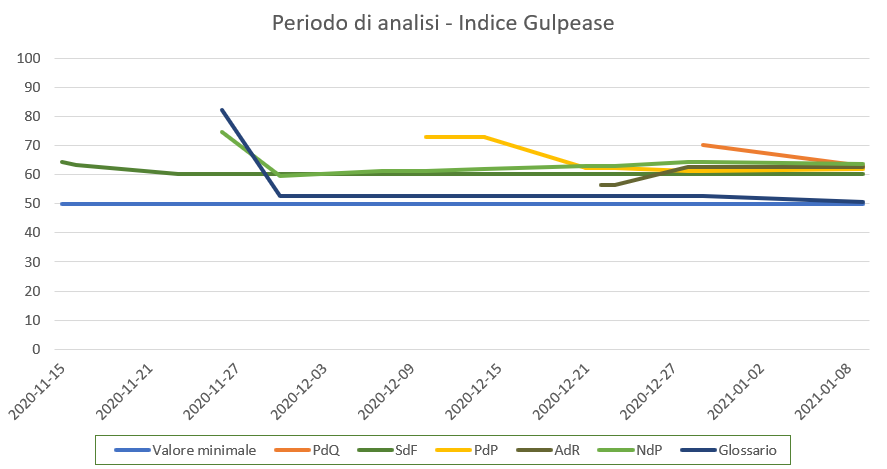
\includegraphics[scale=0.6]{Immagini/GulpeaseAnalisi}\\
	\caption{Indice di Gulpease comprendente l'andamento di tutti i documenti}
	Tutti i documenti soddisfano pienamente il valore minimo di leggibilità esposto in \hyperlink{MPR02}{MPR02}.
	\label{fig:GulpeaseAnalisi}
\end{figure}
Al termine di questo primo periodo si sono calcolati i risultati relativi alla variazione dei costi e della pianificazione. Si sono successivamente stilate due tabelle contenenti i risultati ottenuti.\\Tutti i documenti soddisfano l'obiettivo indicato in \hyperlink{MPR08}{MPR08}.
\begin{table} [H]
	\begin{center}
		\begin{tabular}{|C{6cm}|c|c|}
			\rowcolor{darkblue}
			\textcolor{white}{\textbf{Prodotto}}&
			\textcolor{white}{\textbf{Risultato ottenuto}}&
			\textcolor{white}{\textbf{Valutazione}}\\
			\NdPv{1.0.0} & 0 & Soddisfatto\\ \hline
			\SdFv{1.0.0} & 5 & Soddisfatto\\ \hline
			\AdRv{1.0.0} & 2 & Soddisfatto\\ \hline
			\PdPv{1.0.0} & 4 & Soddisfatto\\ \hline
			\PdQv{1.0.0} & 0 & Soddisfatto\\ \hline
			\Glossariov{1.0.0} & 6 & Soddisfatto\\ \hline
		\end{tabular}
	\end{center}
	\caption{\label{tab:MPR08Analisi}Risultati relativi alla varianza rispetto allo schedule.}
\end{table}\noindent
Nonostante lo sforamento di \textbf{20,00€} si è riusciti a soddisfare pienamente l'obiettivo indicato in \hyperlink{MPR09}{MPR09}.
\begin{table} [H]
	\begin{center}
		\begin{tabular}{|C{6cm}|c|c|}
			\rowcolor{darkblue}
			\textcolor{white}{\textbf{Processo}}&
			\textcolor{white}{\textbf{Risultato ottenuto}}&
			\textcolor{white}{\textbf{Valutazione}}\\
			Differenza dei costi tra il consuntivo di periodo ed il consuntivo finale & -20,00€ & Soddisfatto\\ \hline
		\end{tabular}
	\end{center}
	\caption{\label{tab:MPR09Analisi}Risultati relativi alla varianza dei costi.}
\end{table}\noindent
Nonostante le difficoltà incontrate nello svolgimento del progetto, si è riusciti a soddisfare pienamente l'obiettivo indicato in \hyperlink{MPR10}{MPR10}.
\begin{table} [H]
	\begin{center}
		\begin{tabular}{|C{6cm}|c|c|}
			\rowcolor{darkblue}
			\textcolor{white}{\textbf{Processo}}&
			\textcolor{white}{\textbf{Risultato ottenuto}}&
			\textcolor{white}{\textbf{Valutazione}}\\
			Giorni trascorsi tra l'apertura di una issue e la sua chiusura & 6 & Soddisfatto\\ \hline
		\end{tabular}
	\end{center}
	\caption{\label{tab:MPR10Analisi}Risultati relativi alla varianza dei costi.}
\end{table}

\subsection{Periodo di consolidamento dei requisiti}
In questo periodo di consolidamento dei requisiti, il gruppo {\Gruppo} si è preparato alla presentazione per la Revisione dei Requisiti studiando le varie tecnologie necessarie per l'avanzamento del progetto in modo individuale. Dal momento che non è stata eseguita nessuna operazione di verifica o miglioramento riguardante i documenti redatti, non si è ritenuto di alcuna rilevanza calcolare i risultati delle varie metriche associate alla \glo{qualità} dei documenti prodotti dal gruppo.
 
\subsection{Periodo di progettazione architetturale} \label{ResocontoPArchitetturale}
Durante il periodo di progettazione architetturale, come nel periodo precedente, i documenti redatti da presentare in ingresso alla \glo{\textbf{RP}} sono stati sottoposti a verifica secondo i criteri definiti nelle \NdPv{2.0}. In questo periodo sono stati valutati attraverso verifica anche i vari processi istanziati.
\subsubsection{Esiti verifica}
\myparagraph{Documentazione}
Di seguito si riportano gli esiti delle metriche relative alla documentazione.
\begin{figure}[h]
	\centering
	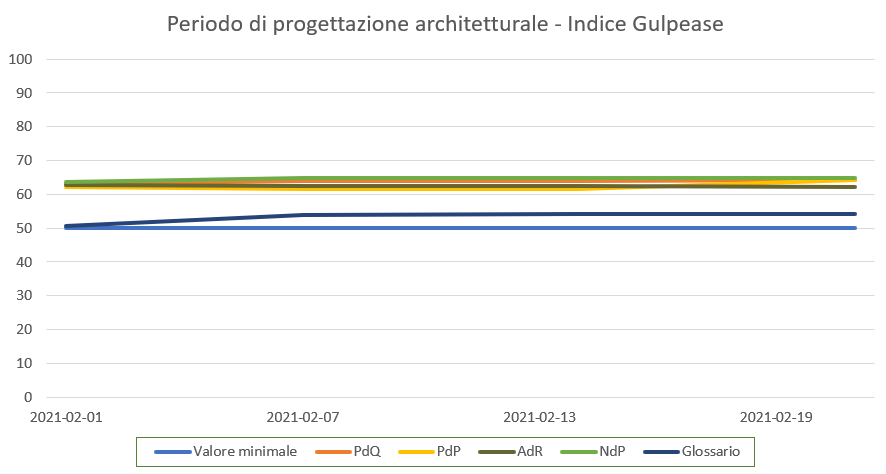
\includegraphics[scale=0.5]{Immagini/GulpeaseProgettazioneArchitetturale}\\
	\caption{Indice di Gulpease}
	\label{fig:GulpeasePArchitetturale}
\end{figure}
\begin{figure}[h]
	\centering
	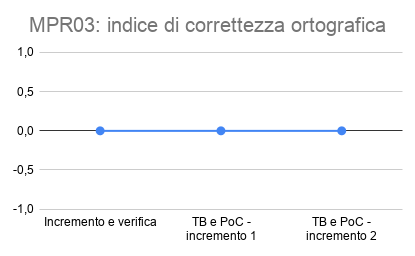
\includegraphics[scale=0.6]{Immagini/MPR03_cortografica}\\
	\caption{Correttezza ortografica documenti progettazione architetturale}
	\label{fig:CortOrtograficaPArchitetturale}
\end{figure}
\\
\myparagraph{Pianificazione}
Di seguito si riportano gli esiti delle metriche relative alla pianificazione.
\begin{figure}[h!]
	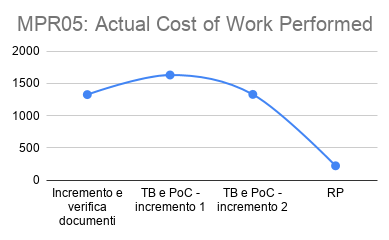
\includegraphics[scale=0.6]{Immagini/ACWP_PArchitetturale.png}\quad
	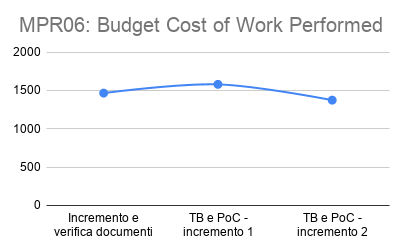
\includegraphics[scale=0.6]{Immagini/BCWP_PArchitetturale.png}
	\caption{ACWP e BCWP progettazione architetturale}
	\label{fig:BCWP_PArchitetturale}
\end{figure}
\begin{figure}[h!]
	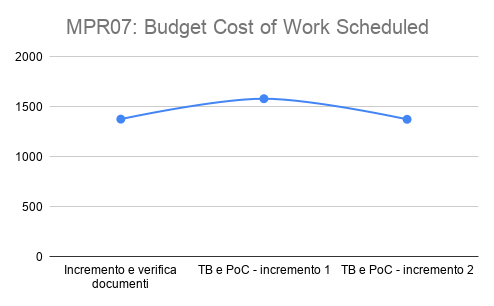
\includegraphics[scale=0.5]{Immagini/BCWS_PArchitetturale.png}\quad
 	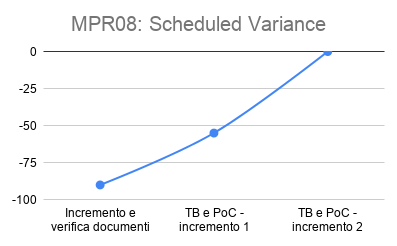
\includegraphics[scale=0.6]{Immagini/SV_PArchitetturale.png}
 	\caption{BCWS e SV progettazione architetturale}
 	\label{fig:SV_PArchitetturale}
\end{figure}
\begin{figure}[h!]
	\centering
	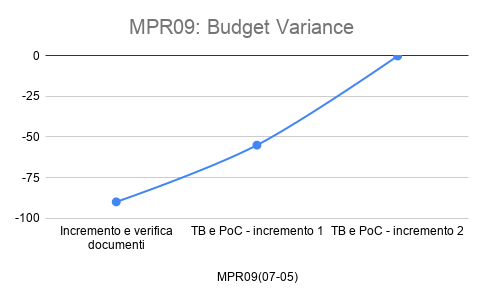
\includegraphics[scale=0.6]{Immagini/BV_PArchitetturale.png}
	\caption{BV progettazione architetturale}
	\label{fig:BV_PArchitetturale}
\end{figure}
\myparagraph{Miglioramento del processo}
Di seguito si riportano gli esiti delle metriche relative al miglioramento del processo.
\begin{figure}[h!]
	\centering
	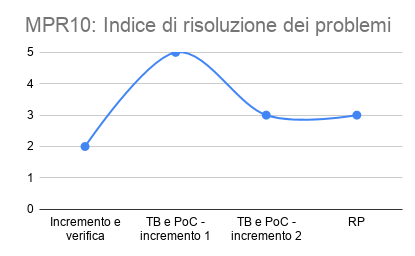
\includegraphics[scale=0.6]{Immagini/MPR10_rproblemi.png}
	\caption{Risoluzione problemi progettazione architetturale}
	\label{fig:MPR10}
\end{figure}

\subsection{Periodo di progettazione di dettaglio e codifica} \label{ResocontoPDettaglio}
Durante il periodo di progettazione di dettaglio, come nel periodo precedente, i documenti redatti da presentare in ingresso alla \glo{\textbf{RQ}} sono stati sottoposti a verifica secondo i criteri definiti nelle \NdPv{3.0}. In questo periodo sono stati valutati attraverso verifica anche i vari processi istanziati.
\subsubsection{Esiti verifica}
\myparagraph{Documentazione}
Di seguito si riportano gli esiti delle metriche relative alla documentazione.
%\begin{figure}[h]
%	\centering
%	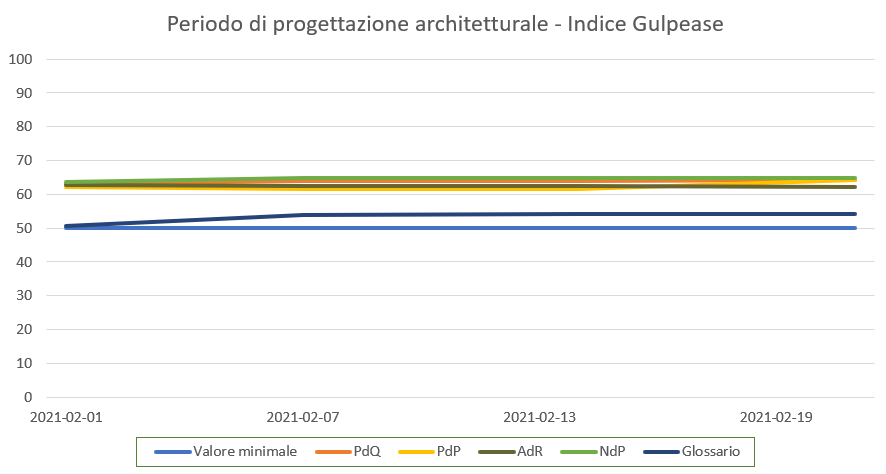
\includegraphics[scale=0.5]{Immagini/GulpeaseProgettazioneArchitetturale}\\
%	\caption{Indice di Gulpease}
%	\label{fig:GulpeasePDettaglio}
%\end{figure}
\begin{figure}[h]
	\centering
	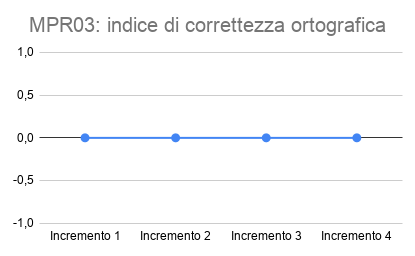
\includegraphics[scale=0.6]{Immagini/MPR03_cortograficadettaglio.png}\\
	\caption{Correttezza ortografica documenti progettazione di dettaglio e codifica}
	\label{fig:CortOrtograficaPDettaglio}
\end{figure}
\\
\myparagraph{Pianificazione}
Di seguito si riportano gli esiti delle metriche relative alla pianificazione.
\begin{figure}[h!]
	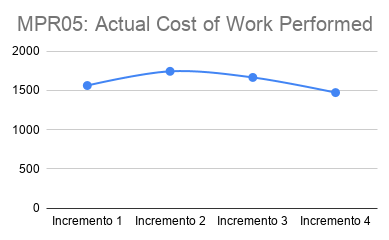
\includegraphics[scale=0.6]{Immagini/ACWP_PDettaglio.png}\quad
	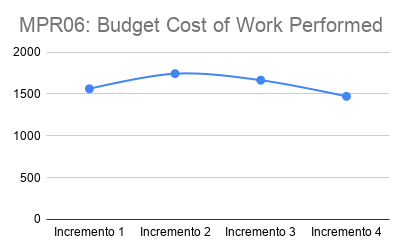
\includegraphics[scale=0.6]{Immagini/BCWP_PDettaglio.png}
	\caption{ACWP e BCWP progettazione di dettaglio e codifica}
	\label{fig:BCWP_PDettaglio}
\end{figure}
\begin{figure}[h!]
	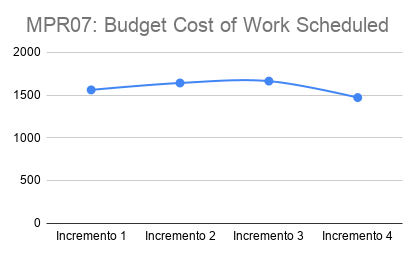
\includegraphics[scale=0.5]{Immagini/BCWS_PDettaglio.png}\quad
	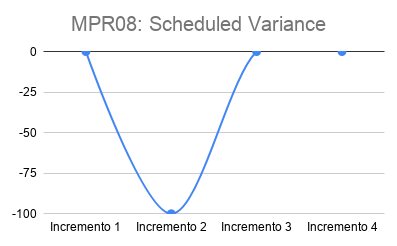
\includegraphics[scale=0.6]{Immagini/SV_PDettaglio.png}
	\caption{BCWS e SV progettazione di dettaglio e codifica}
	\label{fig:SV_PDettaglio}
\end{figure}
\begin{figure}[h!]
	\centering
	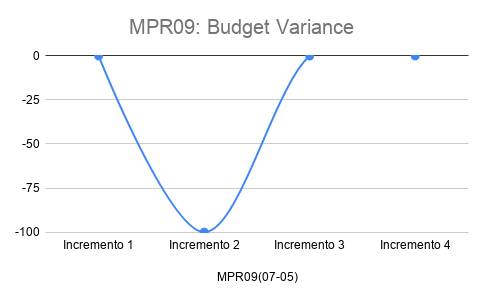
\includegraphics[scale=0.6]{Immagini/BV_PDettaglio.png}
	\caption{BV progettazione di dettaglio e codifica}
	\label{fig:BV_PDettaglio}
\end{figure}
\myparagraph{Codifica}
Di seguito si riportano gli esiti delle metriche relative alla pianificazione.
\begin{figure}[h!]
	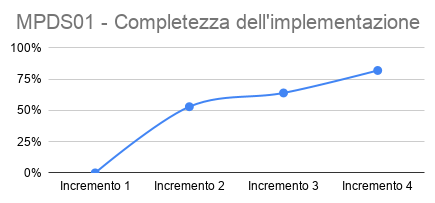
\includegraphics[scale=0.6]{Immagini/MPDS01_CompletezzaImpl.png}\quad
	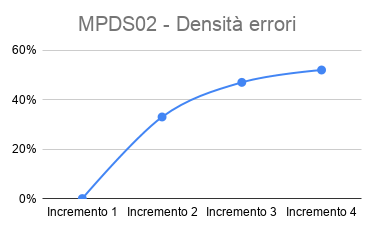
\includegraphics[scale=0.6]{Immagini/MPDS02_DErrori.png}
	\caption{Correttezza dell'implementazione e densità degli errori}
	\label{fig:DensitàErr}
\end{figure}
\begin{figure}[h!]
	\centering
	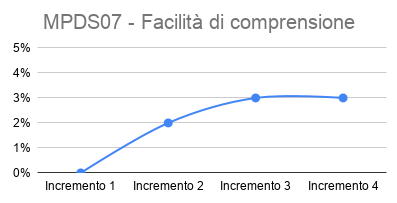
\includegraphics[scale=0.6]{Immagini/MPDS07_FComprensione.png}
	\caption{Facilità di comprensione del codice}
	\label{fig:FacilitàCodice}
\end{figure}

\myparagraph{Miglioramento del processo}
Di seguito si riportano gli esiti delle metriche relative al miglioramento del processo.
\begin{figure}[h]
	\centering
	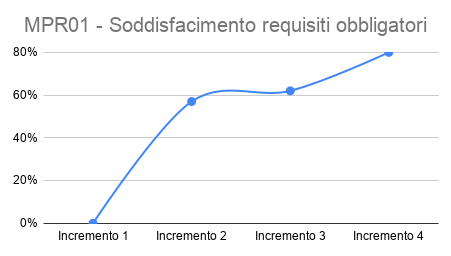
\includegraphics[scale=0.6]{Immagini/MPR01_RObbligatori.png}
		\caption{Soddisfacimento requisiti obbligatori}
		\label{fig:MPR01}
\end{figure}
\begin{figure}[h!]
	\centering
	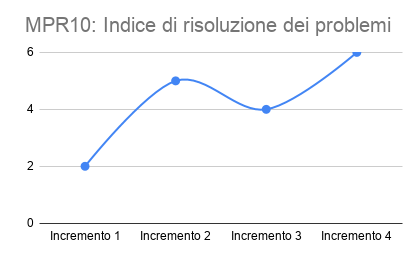
\includegraphics[scale=0.6]{Immagini/MPR10_rproblemidettaglio.png}
	\caption{Risoluzione problemi progettazione di dettaglio e codifica}
	\label{fig:MPR10codifica}
\end{figure}
\newpage

\section{Lista di Controllo}
\label{lista_controllo}
Gli errori più frequenti riscontrati durante la verifica della documentazione si suddividono in:
\begin{itemize}
	\item \textbf{Errori ortografici:}
	\begin{itemize}
		\item Errori di battitura e/o distrazione;
		\item Assenza o uso improprio della punteggiatura;
		\item Mancata concordanza tra le parti variabili del discorso.
	\end{itemize}
	\item \textbf{Errori grammaticali:}
	\begin{itemize}
		\item Errata coniugazione dei verbi;
		\item Discordanza tra le persone utilizzate, si passa da una discorso impersonale alla prima persona plurale e viceversa.
	\end{itemize}
	\item \textbf{Errori visuali:}
	\begin{itemize}
		\item Mancanza di grafici;
		\item Presenza di grafici non aggiornati con la versione corrente del documento.
	\end{itemize}
	\item \textbf{Errori rispetto a quanto definito nelle Norme di Progetto:}
	\begin{itemize}
		\item Mancanza dei caratteri ";" e "." alla fine di ogni voce di un elenco puntato;
		\item Mancato uso del grassetto per le voci di un elenco puntato;
		\item Uso della prima lettera minuscola per indicare i nomi propri dei documenti e delle figure professionali;
		\item Mancato uso del corsivo nel momento in cui ci si riferisce a nomi propri di documenti, figure professionali o termini tecnici.
	\end{itemize}
	\item \textbf{Errori relativi al glossario:}
	\begin{itemize}
		\item Mancata individuazione di termini che risultano ambigui;
		\item Presenza dell'apice $^G$ in parole che non ne hanno bisogno o già segnate nella medesima sezione.
	\end{itemize}
	\item \textbf{Template e comandi:}
	\begin{itemize}
		\item Assenza dei comandi appositamente definiti per semplificare, velocizzare e standardizzare la stesura dei documenti.
	\end{itemize}
\end{itemize}
\newpage

\appendix
\section{Valutazioni per il miglioramento}
\label{miglioramento}
Di seguito viene riportata la valutazione fatta dal gruppo {\Gruppo} riguardo il lavoro svolto durante l'\glo{attività} appena conclusa. Lo scopo di questa scelta è far emergere tutte le problematiche sorte fino ad ora e poter procedere ad una loro risoluzione \glo{efficiente} così da evitare che si verifichino nuovamente in futuro.
I problemi analizzati riguardano:
\begin{itemize}
	\item \textbf{Organizzazione:} criticità relative all'organizzazione e alla comunicazione interna del gruppo;
	\item \textbf{Ruoli:} criticità riguardanti il corretto svolgimento di un ruolo;
	\item \textbf{Strumenti:} criticità relative all'uso degli strumenti scelti.
\end{itemize}
Per trattare ogni punto sopra descritto, è fondamentale l'autovalutazione di ciascun membro del gruppo, non essendo presente una figura esterna che possa valutare in modo oggettivo le criticità. Questo metodo ha permesso al gruppo di migliorare progressivamente la \glo{qualità} del lavoro. La sezione è al momento incompleta, verrà aggiornata con l’avanzamento del lavoro riportando nuove problematiche, ogni qual volta esse dovessero verificarsi. Per fornire valutazioni facilmente leggibili e consultabili esse sono organizzate mediante tabelle la cui struttura è stabilita in \NdPv{1.0.0}.
\subsection{Revisione dei requisiti}
\subsubsection{Valutazioni sull'organizzazione}
\begin{itemize}
	\item \textbf{Problema:} La difficoltà maggiore è stata quella di entrare nell'ottica del progetto e del lavoro di gruppo abituandosi ai cambi di ruolo e ai compiti da svolgere coordinandosi con gli altri membri del gruppo.\\
	\textbf{Soluzione proposta:} I membri del gruppo si sono incontrati e si è organizzato il lavoro dopo aver studiato il \glo{capitolato} e i documenti indicati nei riferimenti normativi. Ciascun componente del team ha avuto modo di ricoprire ogni ruolo attivo fino ad ora, perciò risulterà meno impegnativo in futuro rispettare la rotazione dei ruoli imposta nel \PdPv{1.0.0}.
	\item \textbf{Problema:} Le \glo{issues} create richiedevano dei compiti che si sovrapponevano tra loro, rischiando di effettuare più volte un lavoro inutilmente.\\
	\textbf{Soluzione proposta:} Ogni membro si impegnerà a creare issue più precise e circoscritte assegnandola a sè stesso e, nel caso fosse necessario, al membro del gruppo che lo aiuta nel lavoro.
	\item \textbf{Problema:} Visti i numerosi impegni di ogni componente, durante le prime settimane si è notata una certa difficoltà nell'organizzare gli incontri in modo che fossero presenti tutti.\\
	\textbf{Soluzione proposta:} Si è deciso di utilizzare un calendario condiviso per evidenziare gli impegni di ciascun membro del team. Alla fine di ogni incontro, si decide la data della possibile riunione successiva.
\end{itemize}
\subsubsection{Valutazioni sui ruoli}
\myparagraph{Responsabile di progetto}
\begin{itemize}
	\item \textbf{Problema:} La principale difficoltà di chi ha ricoperto questo ruolo è stata la suddivisione del lavoro in maniera equa ed omogenea provocando una serie di ridistribuzioni degli incarichi tra i vari membri.\\
	\textbf{Soluzione proposta:} Per ridurre il possibile ritardo che si sarebbe potuto presentare, il gruppo ha deciso di dedicare del tempo ad analizzare la quantità di lavoro richiesta così da assegnare con più attenzione i compiti ai vari membri del gruppo. Questo è stato reso possibile usando lo strumento di \glo{ITS} offerto da \glo{GitHub}.
\end{itemize}
\myparagraph{Analista}
\begin{itemize}
	\item \textbf{Problema:} Data l'inesperienza da parte degli \textit{Analisti}, il tracciamento dei requisiti e l'individuazione dei casi d'uso hanno richiesto più ore del previsto, come indicato anche all'interno del \PdPv{1.0.0}.\\
	\textbf{Soluzione proposta:} Dopo aver studiato in maniera autonoma l'argomento, il gruppo ha deciso di dedicare del tempo aggiuntivo per analizzare meglio i casi d’uso da modellare e le tecnologie da impiegare.
\end{itemize}
\myparagraph{Verificatore}
\begin{itemize}
	\item \textbf{Problema:} La verifica è stata svolta in maniera non costante all'inizio e questo ha provocato una mole di documenti da verificare più ampia del previsto incontrando anche contraddizioni di contenuto e struttura tra i diversi documenti.\\
	\textbf{Soluzione proposta:} Una pianificazione migliore del lavoro da svolgere ha aiutato in corso d’opera a evitare che questo succedesse nuovamente. Il gruppo ha poi deciso di dedicare del tempo per analizzare meglio i contenuti di tutti i singoli documenti per evitare l’insorgere di contraddizioni tra gli stessi.
\end{itemize}
\subsubsection{Valutazioni sugli strumenti}
\myparagraph{GitHub}
\begin{itemize}
	\item \textbf{Problema:} Si sono riscontrati diverse difficoltà, specialmente nel periodo iniziale, dovute alla scarsa esperienza di alcuni membri del gruppo nell'utilizzo di tale strumento.\\
	\textbf{Soluzione proposta:} I membri carenti nell'uso di GitHub hanno effettuato un approfondito lavoro individuale per sanare le proprie mancanze.
\end{itemize}
\myparagraph{\LaTeX}
\begin{itemize}
	\item \textbf{Problema:} Per l’inesperienza della quasi totalità dei membri del gruppo all'utilizzo di questo strumento, si sono riscontrate diverse difficoltà specialmente nell'inserimento di figure e nello redarre un template comune per tutti i documenti.\\
	\textbf{Soluzione proposta:} Per risolvere in breve tempo questa problematica, si è deciso di dedicare parte delle prime settimane per apprendere e approfondire l’utilizzo di \LaTeX.
\end{itemize}
\subsection{Revisione di progettazione}
\subsubsection{Valutazioni sull'organizzazione}
\begin{itemize}
	\item \textbf{Problema:} Le attività relative al progetto si sono sovrapposte con gli impegni degli esami universitari. Diversi membri del gruppo hanno tralasciato quasi del tutto le attività di progetto; questo ha portato ad un pesante rallentamento dello sviluppo del prodotto.\\
	\textbf{Soluzione proposta:} I membri meno occupati dalle prove universitarie hanno cercato di far progredire lo sviluppo occupandosi delle parti che non richiedevano il coinvolgimento del gruppo nel suo complesso. Tutti si sono impegnati a dare il proprio contributo nonostante la sessione d'esami; i membri momentaneamente inattivi erano costantemente aggiornati mediante i canali di comunicazione adottati dal gruppo.
\end{itemize}
\subsubsection{Valutazioni sui ruoli}
\myparagraph{Analista}
\begin{itemize}
	\item \textbf{Problema:} Durante lo sviluppo del \glo{PoC} sono emersi nuovi requisiti e si è vista la necessità di dettagliare maggiormente quanto già descritto all'interno dell'{\AdR}. In seguito ad un incontro sostenuto con il {\CR}, sono risultate evidenti altre imprecisioni in requisiti già individuati precedentemente portando ad una sostanziale ristrutturazione del documento stesso.\\
	\textbf{Soluzione proposta:} Gli \textit{Analisti} hanno dovuto rivedere con maggiore attenzione il lavoro svolto nel precedente periodo e correggere gli errori. Dopo un'analisi più approfondita e consapevole; sono stati di grande aiuto il confronto avuto con {\Proponente} e lo studio più approfondito delle tecnologie coinvolte nello sviluppo del progetto.
\end{itemize}
\myparagraph{Progettista}
\begin{itemize}
	\item \textbf{Problema:} A causa della totale inesperienza nel ruolo, i \textit{Progettisti} hanno trovato molte avversità nell'individuare l'architettura ottimale per il prodotto richiesto.\\
	\textbf{Soluzione proposta:} Vista l'intenzione di costruire un prodotto in modo incrementale e quindi di mantenere il più invariato possibile quanto sviluppato al termine di questo periodo, i \textit{Progettisti} hanno dovuto approfondire maggiormente le proprie conoscienze sul settore.
\end{itemize}
\myparagraph{Programmatore}
\begin{itemize}
	\item \textbf{Problema:} Data la totale inesperienza del gruppo nel lavorare con le tecnologie coinvolte, i \textit{Programmatori} hanno incontrato diverse difficoltà nell'impiego dei linguaggi e delle tecnologie richieste; è risultato inoltre complicato anche il dover integrare i vari microservizi sviluppati.\\
	\textbf{Soluzione proposta:} I \textit{Programmatori} hanno colmato le mancanze rilevate tramite un ulteriore periodo di formazione personale e l'esercizio pratico con le tecnologie in uso.
\end{itemize}
\newpage

\section{Esiti delle revisioni}
\label{esito}
Il gruppo \Gruppo\ ha deciso di dedicare alcuni incontri per discutere sulla valutazione critica del lavoro svolto fino a quel momento in seguito alla pubblicazione delle osservazioni da parte dei committenti e di \Proponente\, oltre alle relative correzioni da apportare ai documenti. È importante riportare e tener traccia delle modifiche svolte per ogni osservazione ricevuta. In questo modo si ha sempre sotto controllo il lavoro svolto dai membri del gruppo e definire una possibile soluzione in maniera univoca. Per dare una struttura coerente con lo stile del documento che faciliti l'individuazione della possibile soluzione abbiamo adottato il formato tabellare.
\subsection{Revisione dei requisiti}
\centering
	\begin{longtable}{|C{4cm}|C{8cm}|c|}
		\caption{\label{tab:Criticità}Miglioramenti apportati in seguito alla Revisione dei requisiti.}\\
		\rowcolor{darkblue}
		\textcolor{white}{\textbf{Osservazione}}&
		\textcolor{white}{\textbf{Soluzione adottata}}&
		\textcolor{white}{\textbf{ID}}\\ \hline
		\rowcolor{darkblue}
		\multicolumn{3}{|c|}{\textcolor{white}{\textbf{Criticità generali}}}\\ \hline
		Insufficiente attenzione nella stesura e nella verifica dei documenti. & Il team ha cercato di migliorare il procedimento di verifica continua eseguendo inoltre le operazioni di verifica con maggior cura. & CAVE01\\ \hline %1-2-3-4
		"Scatto" di versione in un prodotto soggetto a manutenzione dovrebbe essere associato solo a modifiche verificate e validate. & Ad ogni cambiamento inserito nel registro delle modifiche viene svolta un'\glo{attività} di verifica. I membri del gruppo hanno inoltre deciso di eliminare il terzo valore presente nella versione in modo da indicare con maggiore attenzione che il documento è effettivamente stato verificato e validato. & CADO01\\ \hline %5
		\rowcolor{darkblue}
		\multicolumn{3}{|c|}{\textcolor{white}{\textbf{Piano di progetto}}}\\ \hline
		Adottato un modello di sviluppo ibrido difficile da governare e decifrare. & La stesura dei documenti deve rispecchiare maggiormente la scelta di adottare il modello di sviluppo incrementale inserendo all'interno del \PdP\ i rischi associati a tale modello e le possibili soluzioni. & CPD01\\ \hline %2
		Il preventivo a finire è un esercizio contabile che non mostra cambiamenti alla pianificazione iniziale. & È possibile inserire una colonna con gli sforamenti avvenuti durante il procedimento di sviluppo. Il gruppo ha deciso poi di scrivere nella sezione della pianificazione \textbf{come} e \textbf{cosa} è cambiato rispetto alla pianificazione iniziale col passare del tempo. & CAPN01\\ \hline %1
		\rowcolor{darkblue}
		\multicolumn{3}{|c|}{\textcolor{white}{\textbf{Analisi dei requisiti}}}\\ \hline
		Imprecisioni tecniche nel disegno dei diagrammi dei casi d’uso. & A seguito di uno studio più approfondito e ad una discussione con \CR{}, i diagrammi in questione sono stati corretti. & CPD02\\ \hline %4-5-6-7-8
		Da approfondire i requisiti funzionali. & Il team ha eseguito un'analisi più profonda del \glo{capitolato} e si sono fissate le metriche per verificare la soddisfazioni di questi. & CAVE02\\ \hline %11
		Insufficiente attenzione nella stesura del documento. & Alcune sezioni e sotto-sezioni inserite all'interno dell'\AdR\ sarebbero dovute essere presenti invece in altri documenti, di conseguenza sono state eliminate dal documento di partenza e trascritte nei documenti più appropriati. Sistemata la numerazione dei sotto-casi d'uso per renderla più coerente con la gerarchia individuata. & CPD03\\ \hline %2-12
		Amministratore come ruolo del sistema. & L'amministratore è stato rimosso dagli attori dal momento che tutte le operazioni che questo può compiere non vengono gestite dalla piattaforma \NomeProgetto, ma dalla \glo{dashboard} di \glo{AWS} & CPAN01\\ \hline %1
		\rowcolor{darkblue}
		\multicolumn{3}{|c|}{\textcolor{white}{\textbf{Norme di progetto}}}\\ \hline
		Presenza di circolarità di riferimento all'inizio delle \NdP\. & Rimossi i riferimenti che causavano il ciclo presenti nel \PdP\ e nel \PdQ\. & CPD04\\ \hline %1
		\rowcolor{darkblue}
		\multicolumn{3}{|c|}{\textcolor{white}{\textbf{Piano di qualifica}}}\\ \hline
		Insufficiente allineamento tra le \NdP\ e il \PdQ rispetto agli obiettivi di \glo{qualità}. & Suddivisi i vari processi individuati all'interno del \PdQ\ in \textbf{processi primari}, \textbf{processi di supporto} e \textbf{processi organizzativi}. Corretta la definizione degli obiettivi di qualità e il metodo con cui calcolare le varie metriche all'interno delle \NdP\. Nel \PdQ è stato aggiunto un "cruscotto" che restituisce una valutazione aggiornata sul raggiungimento degli obiettivi prefissati. & CPD05\\ \hline %1
		Le metriche che si è deciso di adottare non vanno relegate in una appendice dedicata. & Riorganizzata la struttura del \PdQ\. & CPD06\\ \hline %2
	\end{longtable}
%\caption{\label{tab:Criticità}Miglioramenti apportati in seguito alla Revisione dei requisiti.}
\end{document}